\part{Représentation des connaissances et raisonnement}
\pagebreak

\chapter{Logique propositionnel}
\section{Vocabulaire}
Les $Logiques propositionnel$ sont définit via les symboles suivant:\\
$\top, \bot, C, \neg C, C \wedge C, C \vee C, C \Rightarrow C$ \\

\begin{description}
\item[Littéral] est un atome ou la négation d'un atome
\item[Clause] est une disjonction de littéraux
\item[Cube] est une conjonction de littéraux
\item[CNF] est une forme normal conjonctive (une conjonction de clauses)
\item[DNF] est une forme normal disjonctive (une disjonction de cubes)
\end{description}

\section{cohérence d'un ensemble de clauses}
Soit K un ensemble de clauses pouvant être réduit via les axiomes:
\begin{description}
\item[] $x \vee x \vee y_1 \vee ... y_n \equiv x \vee y_1 \vee ... y_n$
\item[] $x \vee \neg x \vee y_1 \vee ... y_n \equiv `top$
\item[] $x \vee \top \equiv \top$
\item[] $x \vee \bot \equiv x$
\item[] Si K est vide alors K est cohérente
\item[] Si $\bot \in $ K alors K est incohérente
\item[] $K_{x \leftarrow \top}$ est le résultat du remplacement des occurrences de $x$ par $\top$
\item[] $K_{x \leftarrow \bot}$ est le résultat du remplacement des occurrences de $x$ par $\bot$
\end{description}

\chapter{Introduction à la logique de description}
\section{Attributive Language with Complement}

Les $ALC$ sont définit via les symboles suivant:\\
$\top, \bot, C, \neg C, C \sqcap C, C \sqcup C, \forall r.C, \exists r.C$\\

\subsection{Sémantique}
Tuple $\iota =_{def} \langle \delta^I, .^I \rangle$ où
\begin{description}
\item[$\delta^I$] est le domaine (ou un ensemble d'objets)
\item[$.^I$] est une fonction d'interprétation tel que 
\begin{description}
\item[] $A^I \subseteq \Delta^I$
\item[] $r^I \subseteq \Delta^I$ x $ \Delta^I$
\item[] $a^I \in \Delta^I$
\end{description}
\item[$\top^I$] $=_{def} \Delta^I$
\item[$\bot^I$] $=_{def} \theta$
\item[$(\neg C)^I$] $=_{def} \Delta^I \\ C^I$
\item[$C \sqcap D)^I$] $=_{def} C^I \cap C^I$
\item[$C \sqcup D)^I$] $=_{def} C^I \cup C^I$
\item[$\exists r.C)^I$] $=_{def} \{ x \in \Delta^I | r^I(x) \cap C^I \neq \theta \}$
\item[$\forall r.C)^I$] $=_{def} \{ x \in \Delta^I | r^I(x) \subseteq C^I \}$
\end{description}

\subsection{Propriétés}
\begin{multicols}{2}
[
Pour toutes les interprétations $\iota = \langle \Delta^I, .^I \rangle$, et pour tout $C,D \in \ell_{ALC}$:
]
\begin{description}
\item[$(\neg \neg C)^I$] $= C^I$
\item[$(\neg (C \sqcap D))^I$] $= ( \neg C \sqcup \neg D)^I$
\item[$(\neg (C \sqcup D))^I$] $= ( \neg C \sqcap \neg D)^I$
\item[$(\neg \forall r.C)^I$] $= (\exists r.\neg C)^I$
\item[$(\neg \exists r.C)^I$] $= (\forall r.\neg C)^I$
\item[$\exists r. \bot $] $\equiv \bot $
\item[$\forall r. \top $] $\equiv \top $
\end{description}
\end{multicols}

\section{Logique de description}
Définit via les symboles suivant:\\
$\ell_{ALC}, C \sqsubseteq C, \sqsupseteq C$\\

\subsection{Sémantique}
\begin{description}
\item[$\iota \Vdash C \sqsubseteq D$] $(\iota satisfait C \sqsubseteq D)$ si $C^I \subseteq D^I$
\item[$\iota \Vdash C \equiv D$] $\iota \Vdash C \sqsubseteq D$ et $\iota \Vdash C \sqsupseteq D$
\end{description}

\subsection{Assertions}
\begin{description}
\item[$a : C$] $a$ est une instance de $C$
\item[$(a,b) : r$] $a$ et $b$ sont attaché avec la relation $r$
\end{description}

\section{TBoxes et ABoxes}
Soit une base de connaissance $KB = \langle T,A \rangle$ où:
\begin{description}
\item[$T = $] 
$\begin{cases}
\cblue{EmpStud} \equiv \cblue{Student} \sqcap \cblue{Employee} \\
\cblue{Student} \sqcap \neg \cblue{Employee} \sqsubseteq \neg \exists  \cviolet{pays}.\cblue{Tax} \\
\cblue{EmpStud} \sqcap \neg \cblue{Parent} \sqsubseteq \exists  \cviolet{pays}.\cblue{Tax} \\
\cblue{EmpStud} \sqcap \cblue{Parent} \sqsubseteq \neg \exists \cviolet{pays}.\cblue{Tax} \\
\exists \cviolet{worksFor}.\cblue{Company} \sqsubseteq \cblue{Employee}
\end{cases}$
\item[$A = $]
$\begin{cases}
\corange{ibm}: \cblue{Company} \\
\corange{mary} : \cblue{Parent} \\
\corange{john}: \cblue{EmpStud} \\
\corange{(john,ibm)}:\cviolet{workFor} \\
\end{cases}$
\end{description}

\subsection{Subsumption}
D'après la TBoxes et la ABoxes ci dessus, dire que A subsume B c'est dire que A est plus spécifique que B:
\begin{description}
\item[] Does $\cblue{EmpStud}$ subsume $\cblue{Student} \sqcap \cblue{Employe}$ ? : yes
\item[] Does $\cblue{Student} \sqcap \cblue{Parent}$ subsume $\cblue{EmpStud} \sqcap \cblue{Parent}$ ? : yes
\item[] Does $\exists \cviolet{pays}.\bot$ subsume $\cblue{EmpStud}$ ? : No
\end{description}

\subsection{Classification}
Les schémas de classification aide pour trouver les subsumptions:

\begin{tikzpicture}[->,>=stealth',shorten >=1pt,auto,node distance=3cm,
                    semithick]
  \tikzstyle{every state}=[fill=white,draw=none,text=black]

  \node[state] 		   (A)                    {$\cblue{EmpStud}$};
  \node[state]         (B) [below left of=A]  {$\cblue{Student}$};
  \node[state]         (C) [below right of=A] {$\cblue{Employes}$};
  \node[state]         (D) [right of=C]       {$\cblue{Tax}$};
  \node[state]         (E) [right of=D]       {$\cblue{Company}$};
  \node[state]         (F) [right of=E]       {$\cblue{Parent}$};

  \path (A) edge              node {} (B)
            edge              node {} (C);
\end{tikzpicture}

\subsection{Instance checking}
On n'a
\begin{description}
\item[$\corange{ibm}$] est une instance de $\cblue{Company}$
\item[$\corange{mary}$] est une instance de $\cblue{Parent}$
\item[$\corange{john}$] est une instance de $\cblue{EmpStud, Student, Employee}$
\item[$\corange{john}$] n'est pas une instance de $\cblue{\neg Parent}$
\item[$\corange{(john,ibm)}$] est une instance de $\cviolet{workFor}$
\end{description}

\subsection{Retrieval}
\begin{description}
\item[$\cblue{Student}$] $? \{ \corange{john} \}$
\item[$\neg \exists \cviolet{pays}.\cblue{Tax}$] $? \{ \corange{mary} \}$
\item[$\neg ( \neg \cblue{Employes} \sqcap \exists \cviolet{pays}.\cblue{Tax})$] $? \{ \corange{john}, \corange{mary} \}$
\item[$\forall \cviolet{worksFor}.\cblue{Company}$] $? \{ \}$
\item[$\cblue{Employee} \sqcup \forall \cviolet{pays} . \neg \cblue{Tax} \sqcup \cblue{Company}$] $? \{ \corange{ibm}, \corange{john}, \corange{mary} \}$
\item[$\neg \cblue{Tax} \sqcup \exists \cviolet{pays} . \bot \sqcup \forall \cviolet{workdFor} . \forall \cviolet{pays} . \top$] $? \{ \corange{ibm}, \corange{john}, \corange{mary} \}$
\end{description}

\subsection{Equivalance of concept}
\begin{description}
\item[Are $\cblue{Student} \sqcap \cblue{Employee} \sqcap \neg \cblue{EmpStud}$ and $\exists \cviolet{worksFor}.\bot$] équivalent? $Yes$
\item[Are $\cblue{Student} \sqcap \forall \cviolet{worksFor}.\neg \cblue{Company}$ and $\cblue{Student} \sqcap \neg \cblue{Employee}$] équivalent? $No$
\end{description}

\subsection{Concept satisfiability}
\begin{description}
\item[$\cblue{EmpStud} \sqcap \cblue{Parent} \sqcap \exists \cviolet{pays}.\top $] satisfiable? $Yep$
\item[$\neg \forall \cviolet{worksFor}.\neg \cblue{Company} \sqcap \neg \cblue{Employee} $] satisfiable? $No$
\item[$\cblue{Employee} \sqcap \cblue{Company} $] satisfiable ? $Yep$
\end{description}

\subsection{ABox consistency}
\begin{description}
\item[Is $A_2 = A \cup \{\corange{john} : \exists \cviolet{worksFor}.\neg \cblue{Company} \} $] consistent wrt $T$ ? : $Yes$
\item[Is $A_3 = A \cup \{\corange{mary} : \exists \cviolet{pays}.\cblue{Tax} \} $] consistent wrt $T$ ? : $No$
\end{description}

\subsection{Réduction et consistance}
Soit $KB = \langle T,A \rangle , C, D \in \iota_{ALC}, a \in I$ and $ a^` $ new in $KB$\\
\begin{description}
\item[Concept subsumption wrt $T$]: $KB \vDash C \sqsubseteq D$ ssi $\langle T, A \cup \{ a^` : C \sqcap \neg D \} \rangle$ est inconsistant
\item[Instance chacking]: $KB \vDash a : C$ ssi $\langle T, A \cup \{ a : \neg C \} \rangle$ est inconsistant
\item[Concept satisfiability wrt $T$]: $C$ est satisfiable wrt $T$ ssi $\langle T,A \cup \{ a^` : C \} \rangle$ est consistent
\end{description}
\begin{description}
\item[$KB \vDash \cblue{EmpStud} \sqcap \cblue{Parent} \sqsubseteq \neg \exists \cviolet{pays}.\cblue{Tax} \sqcap \cblue{Employee} $]?\\ $\ KB \cup \{ \corange{a} : \cblue{EmpStud} \sqcap \cblue{Parent} \sqcap (\exists \cviolet{pays}.\cblue{Tax} \sqcup \neg \cblue{Employee} ) \} \vDash \bot ?,$ for $\corange{a}$ new
\item[$KB \vDash \corange{john} : \cblue{Student} \sqcap \exists \cviolet{empBy}.\top $]?\\  $\ KB \cup \{ \corange{john} : \neg (\cblue{Student} \sqcap \exists \cviolet{empBy}.\top)\} \vDash \bot ?$
\item[Is $\cblue{EmpStud} \sqcap \neg \exists \cviolet{pays}.\cblue{Tax}$ satisfiable wrt $KB$ ]?\\ $\ KB \cup \{ \corange{a} : \cblue{EmpStud} \sqcap \neg \exists \cviolet{pays}.\cblue{Tax} \nvDash \bot ?,$ for $\corange{a}$ new
\end{description}

\chapter{Méthode des Tableau pour les ALC}
\section{Pre processing}
\subsection{Réécriture}
Réécrite chaque:
\begin{description}
\item[] $C \sqsubseteq D$ dans $T$ en $\top \sqsubseteq \neg C \sqcup D$
\item[] $A \sqsubseteq \exists r.B$ en $\top \sqsubseteq \neg A \sqcup \exists r.B$
\end{description}
\ \\
Changer la $KB$ en $NNF$ ($\neg$ occurs only in front of concept names)
\begin{description}
\item[$\neg \neg C$] $\rightarrow C$
\item[$\neg (C \sqcap D)$] $\rightarrow \neg C \sqcup \neg D$
\item[$\neg (C \sqcup D)$] $\rightarrow \neg C \sqcap \neg D$
\item[$\neg (\exists r.C)$] $\rightarrow \forall r.\neg C$
\item[$\neg (\forall r.C)$] $\rightarrow \exists r.\neg C$
\end{description}

\subsection{Vocabulaire}
\begin{description}
\item[Blocage/Blocking] l'apparition d'une boucle infini dans le déroulement de l'algorithme 
\item[Clash] Quand il existe une contradiction d'un noeud feuille vers l'un de ses ascendant
\end{description}

\subsection{Règles d'expansion}
\begin{description}
\item[$\sqsubseteq_{T} -$] rule\\
\begin{description}
\item[Si $a : C \in A, \top \sqsubseteq D \in T$ et $a : D \notin A$] alors\\ $A := A \cup \{ a : D \}$
\end{description}
\item[$\sqcap -$]rule\\
\begin{description}
\item[Si $a : C \sqcap D \in A$ et $\{ a : C, a : D \nsubseteq A$] alors\\ $A := A \cup \{ a : C, a : D\}$
\end{description}
\item[$\sqcup -$]rule\\
\begin{description}
\item[Si $a : C \sqcup D \in A$ et $\{ a : C, a : D \} \cap A = \varnothing$] alors\\ $A := A \cup \{a : E\},$ for some $E \in \{C,D\}$
\end{description}
\item[$\exists -$]rule\\
\begin{description}
\item[Si $a : \exists R.C \in A$ et il n'y a pas de $b$ st $\{(a,b) : R, b : C\} \subseteq A$ et]
\item[$a $ n'est pas en en blocage] alors\\ $A := A \cup \{(a,c) : R,c : C \},$ for $c$ new in $A$
\end{description}
\item[$\forall -$]rule\\
\begin{description}
\item[Si $\{a : \forall R.C, (a,b) : R\} \subseteq A$ et $b : C \notin A$] alors\\ $A := A \cup \{b : C \}$
\end{description}
\end{description}

\section{Exemple}
\begin{description}
\item[$T$] = $\{ A \sqsubseteq \exists r.B \}$ $\equiv$ $\{\top \sqsubseteq \neg A \sqcup \exists r.B \}$
\item[$A$] = $\{a : A \sqcap B, a : \forall r.\forall r.C \}$
\end{description}

\scalebox{0.9}{
\begin{tikzpicture}[sibling distance=10em,
  every node/.style = {scale=1,
    draw=none, align=center}]]
  \node {$\{ \crouge{a : A \sqcap B}, a : \forall r.\forall r.C \}$}
    child { node {$\{ \cviolet{a:A},a:B\}$}
      child { node {$\{a: \neg A \sqcup \exists r.B \}$}
        child { node {$\{ \cviolet{a: \neg A }\}$} }
        child { node {$\{ a : \exists r.B \}$} 
          child { node {$\{ (a,x) : r,x B \}$} 
            child { node {$\{ x : \forall r.C\}$}
              child { node {$\{x : \neg A \sqcup \exists r.B \}$}
                child { node {$\{ x : \neg A \}$} }
                child { node {$\{x : \exists r.B \}$}
                  child { node {$\{(x,y) : r,y B \}$ }
                    child { node {$\{y : C \}$}
                      child { node {$\{ y: \neg A \sqcup \exists r.B \}$}
                        child { node {$\{ y : \neg A \}$} }
                        child { node {$\{ y : \exists r.B \}$}
                          child { node {y est bloqué par z} }
                        }
                      }
                    }
                  }
                }
              }
            }
          } 
       	}
      }
    };
\end{tikzpicture}
}
\pagebreak

\section{Exemple 2}
\begin{description}
\item[$T$] = $\{ A \sqsubseteq \exists r.B \}$ $\equiv$ $\{\top \sqsubseteq \neg A \sqcup \exists r.B \}$
\item[$A$] = $\{ a : A \sqcap B, a : \forall r.(A \sqcap \forall r.A) \}$
\end{description}

\scalebox{0.7}{
\begin{tikzpicture}[sibling distance=10em,
  every node/.style = {scale=1,
    draw=none, align=center}]]
  \node {$\{ \crouge{a : A \sqcap B}, a : \forall r.(A \sqcap \forall r.A) \}$}
    child { node {$\{ \cviolet{a : A}, a : B \}$}
      child { node { $\{ a : \neg A \sqcup \exists r.B \}$ }
	    child { node {$\{ \cviolet{a : \neg A} \}$}}
	    child { node {$\{ a : \exists r.B \}$}
	      child { node {$\{ (a,x) : r,xB \}$}
	        child { node {$\{ x : A \sqcap \forall r.A \}$}
	          child { node {$\{ \cviolet{x : A,} x : \forall r.A \}$} 
	            child { node {$\{ x : \neg A \sqcup \exists r.B \}$ }
				  child { node {$\{ \cviolet{x : \neg A} \}$ } }
				  child { node {$\{ x : \exists r.B \} $}
				    child { node {$\{ (x,y) : r,yB \}$}
	        		  child { node {$\{ y : A \sqcap \forall r.A \}$}
	          		    child { node {$\{ \cviolet{y : A,} y : \forall r.A \}$} 
	            		  child { node {$\{ y : \neg A \sqcup \exists r.B \}$ }
				  			child { node {$\{ \cviolet{y : \neg A} \}$ } }
				  			child { node {$\{ y : \exists r.B \} $}
				  			  child { node { $...InfinitLoop...$ } }
				  			}	            
	           			  }
	          			}
	        		  }
	      			}
				  }	            
	            }
	          }
	        }
	      }
	    }
      }    
    };
\end{tikzpicture}
}

\chapter{Logique presque tout}

Soit le nouvelle opérateur binaire $\Subset$ disent pour $\crouge{presque\ tout}$ A est dans B.\\

\begin{description}
\item[Bonne distribution]:\\
\scalebox{0.5}{
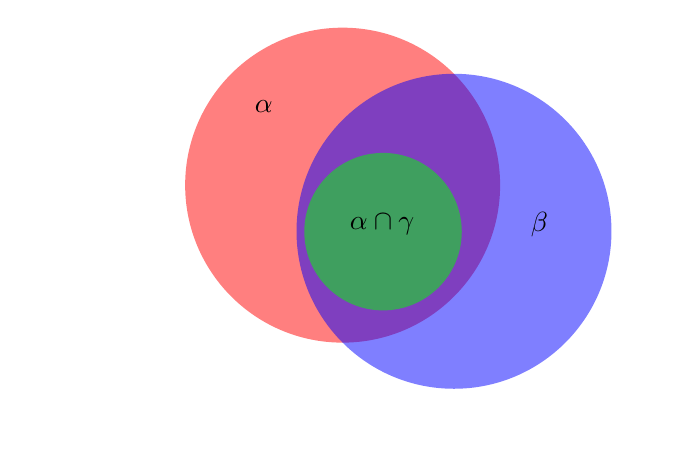
\begin{tikzpicture}
\fill[white](-4,-1) rectangle (4,4);
\fill[opacity=0.5,red] (0,0) ++(90:2) circle (2);
\fill[opacity=0.5,blue] (0,0) ++(45:2) circle (2);
\fill[opacity=0.5,green] (0,0) ++(70:1.5) circle (1);
\node[draw=none] at (-1,3) {$\alpha$};
\node[draw=none] at (2.5,1.5) {$\beta$};
\node[draw=none] at (0.5,1.5) {$\alpha \cap \gamma$};
\end{tikzpicture}}
\item[Mauvaise distribution]:\\
\scalebox{0.5}{
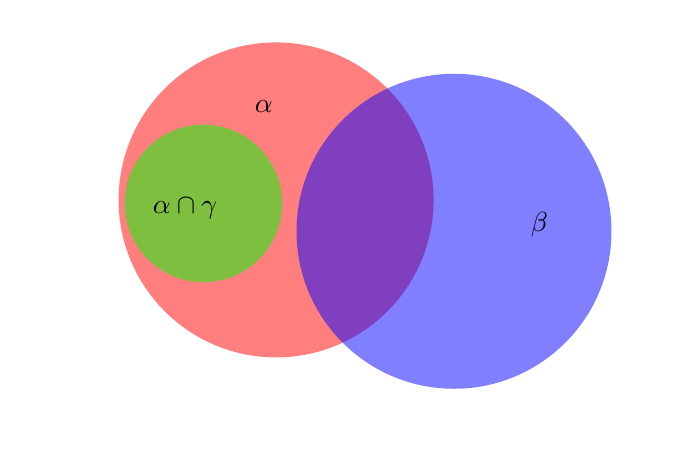
\begin{tikzpicture}
\fill[white](-4,-1) rectangle (4,4);
\fill[opacity=0.5,red] (0,0) ++(115:2) circle (2);
\fill[opacity=0.5,blue] (0,0) ++(45:2) circle (2);
\fill[opacity=0.5,green] (0,0) ++(135:2.5) circle (1);
\node[draw=none] at (-1,3) {$\alpha$};
\node[draw=none] at (2.5,1.5) {$\beta$};
\node[draw=none] at (-2,1.7) {$\alpha \cap \gamma$};
\end{tikzpicture}}
\item[Cas général]:\\
\scalebox{0.5}{
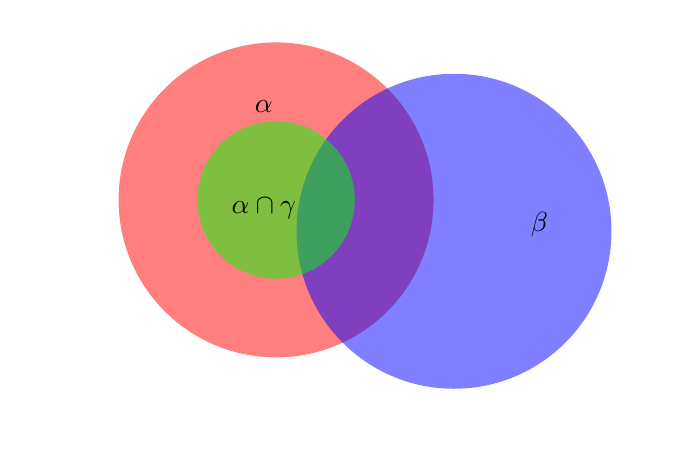
\begin{tikzpicture}
\fill[white](-4,-1) rectangle (4,4);
\fill[opacity=0.5,red] (0,0) ++(115:2) circle (2);
\fill[opacity=0.5,blue] (0,0) ++(45:2) circle (2);
\fill[opacity=0.5,green] (0,0) ++(115:2) circle (1);
\node[draw=none] at (-1,3) {$\alpha$};
\node[draw=none] at (2.5,1.5) {$\beta$};
\node[draw=none] at (-1,1.7) {$\alpha \cap \gamma$};
\end{tikzpicture}}
\end{description}

\section{Système P}
\begin{description}
\item[Réflexivité]:
\begin{description}
\item[Almost all]: $\alpha \almost \alpha$
\item[ensembliste]: $A \Subset A$
\end{description}
\item[Équilibrage à gauche]:
\begin{description}
\item[Almost all]: Si $\models \alpha \Leftrightarrow \beta$ et $\alpha \almost \gamma$ alors $\beta \almost \gamma$
\item[ensembliste]: Si $A = B$ et $A \Subset C$ alors $B \Subset C$
\end{description}
\item[Équilibrage à droite]:
\begin{description}
\item[Almost all]: Si $\alpha \models \beta$ et $\gamma \almost \alpha$ alors $\gamma \almost \beta$
\item[ensembliste]: Si $A \subseteq B$ et $C \Subset A$ alors $C \Subset B$
\end{description}
\item[Coupure]:
\begin{description}
\item[Almost all]: Si $(\alpha \wedge \beta) \almost \gamma$ et $\alpha \almost \beta$ alors $\alpha \almost \gamma$
\item[ensembliste]: Si $(A \cap B) \Subset C$ et $A \Subset B$ alors $A \Subset C$
\end{description}
\item[Monotonie]:
\begin{description}
\item[Almost all]: Si $\alpha \almost \beta$ et $\alpha \almost \gamma$ alors $\alpha \wedge \beta \almost \gamma$
\item[ensembliste]: Si $A \Subset B$ et $A \Subset C$ alors $(A \cap B) \Subset C$
\end{description}
\item[Ou]:
\begin{description}
\item[Almost all]: Si $\alpha \almost \gamma$ et $\beta \almost \gamma$ alors $\alpha \vee \beta \almost \gamma$
\item[ensembliste]: Si $A \Subset C$ et $B \Subset C$ alors $(A \cup B) \Subset C$
\end{description}
\end{description}
\pagebreak
\subsection{Exemple}
Soit:
\begin{description}
\item[$Q$] : être québécoises 
\item[$C$] : être canadiens
\item[$F$] : le fait de parler français 
\item[$A$] : le fait de parler anglais 
\item[$S$] : le fait d'aimer le sirop d'érable
\end{description}
\ \\
\begin{description}
\item[Presque tout les canadiens ne parlent pas le français]: $C \almost \neg F$
\item[Presque tout les québécois parlent le français]: $Q \almost F$
\item[Les québécois aiment le sirop d'érable]: $Q \Rightarrow S \equiv Q \almost S$
\item[Les québécois sont canadiens] $Q \Rightarrow C \equiv Q \almost C$
\end{description}
\ \\
\begin{description}
\item[Presque tout les québécois canadiens parlent le français]\ 
\begin{description}
\item[Nous avons] $Q \almost C$ et $Q \almost F$
\item[Avec la monotonie on obtient] $Q \wedge C \almost F$
\end{description}
\item[Presque tout les québécois canadiens parlent le français ou l'anglais]\ 
\begin{description}
\item[Avec] $Q \wedge C \almost F$
\item[Par ailleurs nous avons] $F \models F \vee A$
\item[Alors via l'équilibrage à droite] $Q \wedge C \almost F \vee A$
\end{description}
\end{description}

\subsection{Caractériser Système P}
Soit la basse de connaissance:
\begin{description}
\item[$\Delta$]
\begin{description}
\item[] $C \Rightarrow \neg F$
\item[] $Q \Rightarrow F$
\end{description}
\item[$W$]
\begin{description}
\item[] $Q \Rightarrow S$
\item[] $Q \Rightarrow C$
\end{description}
\end{description}

\begin{multicols}{2}
[
Pour une formule de type $A \Rightarrow B$ dans $\Delta$ dire si il existe une interprétation qui vérifie $A \Rightarrow B$ et qui satisfait chacune des règles de $\Delta$ et $W$
]
\begin{description}
\item[Pour la formule] $C \Rightarrow \neg F$ est satisfait
\item[$\Delta$]
\begin{description}
\item[] $\corange{C^1} \Rightarrow \neg \cviolet{F^0}$
\item[] $\cblue{Q^0} \Rightarrow \cviolet{F^0}$
\end{description}
\item[$W$]
\begin{description}
\item[] $\cblue{Q^0} \Rightarrow S^s$
\item[] $\cblue{Q^0} \Rightarrow \corange{C^1}$
\end{description}
\end{description}

\begin{description}
\item[Pour la formule] $Q \Rightarrow F$ n'est pas satisfait
\item[$\Delta$]
\begin{description}
\item[] $\corange{C^1} \Rightarrow \neg \cviolet{F^1} \equiv \neg \top \vee \bot$
\item[] $\cblue{Q^1} \Rightarrow \cviolet{F^1}$
\end{description}
\item[$W$]
\begin{description}
\item[] $\cblue{Q^1} \Rightarrow S^s$
\item[] $\cblue{Q^1} \Rightarrow \corange{C^1}$
\end{description}
\end{description}


\end{multicols}

\pagebreak